\documentclass[conference]{IEEEtran}
\IEEEoverridecommandlockouts

\usepackage{amsmath,amssymb,amsfonts}
\usepackage{textcomp}
\usepackage{xcolor}
\usepackage{graphicx}
\usepackage{booktabs}
\usepackage{cite}
\usepackage{url}
\usepackage{tikz}
\usetikzlibrary{shapes.geometric, arrows.meta, positioning, calc}
\usepackage{pgfplots}
\pgfplotsset{compat=1.18}

\def\BibTeX{{\rm B\kern-.05em{\sc i\kern-.025em b}\kern-.08em
    T\kern-.1667em\lower.7ex\hbox{E}\kern-.125emX}}

\begin{document}

\title{Who Writes the Testbench Matters: Auditing False Rejections in LLM-Generated Verilog Testbenches}

\author{\IEEEauthorblockN{Soham Guha}
\IEEEauthorblockA{\textit{School of Computer Engineering} \\
\textit{Kalinga Institute of Industrial Technology (KIIT) Deemed to be University}\\
Bhubaneswar, Odisha, India \\
Email: soham.guha@kiit.ac.in}
}

\maketitle

\begin{abstract}
Closed-loop LLM flows for register-transfer level (RTL) design increasingly let a language model write the testbench that judges a candidate circuit. If that testbench rejects a correct design, the loop is steered away from correct hardware. We audit 1,022 free-form, self-checking Verilog testbenches written by GPT-4o-mini and Gemini Flash-Lite (plus a 20-trial local-model pilot) for 30 VerilogEval-v2 spec-to-RTL problems, and measure how often a testbench that compiles and obeys its output contract nevertheless fails the golden reference design. This \textit{false rejection} occurs in 58.32\% of all trials (596/1,022; problem-level cluster bootstrap 95\% CI [48.69\%, 67.72\%]) and in 60.51\% of testbenches that pass the compile-and-contract gate (596/985). All 1,022 verdicts reproduce exactly when re-simulated under Icarus Verilog~12.0, and \VERILATORABSTRACT. Six prompting conditions---self-testing, an adversarial ``red-team'' prompt with and without the candidate RTL, the same prompts given to the other model, and an independent resample of the self-test---all fall between 55.7\% and 62.9\% ($\chi^2 = 3.15$, $p = 0.68$). In contrast, the identity of the model that writes the testbench is decisive: GPT-4o-mini testbenches falsely reject 74.3\% of the time versus 42.6\% for Gemini Flash-Lite (paired per-problem difference $-31.2$ percentage points, 95\% CI [$-42.6$, $-20.2$]; problem-clustered GEE odds ratio 4.13, [2.50, 6.81]). Once the tester is fixed, the identity of the model that wrote the candidate RTL has no measurable effect, and an adversarial prompt does not reduce---and may slightly increase---false rejections. False rejections are concentrated in sequential circuits (68.0\% vs.\ 33.8\% for combinational) and vary from 0\% to 94\% across problems (ICC $= 0.27$). In 31 of 194 cases where the tester saw a \textit{buggy} candidate, the resulting testbench rejected the golden design while accepting the buggy one. We release the audit scripts and per-trial re-simulation results.
\end{abstract}

\begin{IEEEkeywords}
Hardware verification, large language models, Verilog RTL, testbench generation, false rejection, empirical study.
\end{IEEEkeywords}

\section{Introduction}
Large language models (LLMs) are now routinely evaluated as RTL authors~\cite{liu2023verilogeval, pinckney2024revisiting, lu2024rtllm, blocklove2023chipchat}. Feedback-driven frameworks such as AutoChip~\cite{thakur2023autochip} close the loop by simulating LLM-generated Verilog against a testbench and returning compiler and simulation errors to the model. AutoChip assumes the testbench is supplied and correct; more recent agentic systems remove this assumption by having LLM agents generate the testbench as well~\cite{zhao2024mage, qiu2024autobench, qiu2024correctbench}.

This shift makes the reliability of the testbench a first-order concern. In hardware, escaped functional bugs are expensive~\cite{wile2005verilog}, but the opposite error is also costly inside an automated loop: a testbench that \textit{falsely rejects} a correct design sends the generator into spurious repair iterations and, if its expectations encode a misreading of the specification, actively pushes the design toward that misreading. Whether a second model, a different model family, or an adversarial prompt reduces such errors is an empirical question; it is motivated by evidence that errors of different LLMs are correlated, especially within a provider~\cite{kim2025correlated}, and by multi-agent debate results in reasoning tasks~\cite{du2023debate}.

We audit 1,022 free-form, self-checking Verilog testbenches for 30 VerilogEval-v2 problems~\cite{liu2023verilogeval,pinckney2024revisiting}. Each testbench passes through three gates: (1) it must compile with the golden RTL under Icarus Verilog~12.0 (\texttt{-g2012}) and print exactly one standardized PASS/FAIL line before \texttt{\$finish}; (2) it must report PASS on the golden reference RTL; and (3) it must report FAIL on an inverted-output version of the golden RTL (non-vacuity). A trial is a \textit{false rejection} when
\begin{equation}
F_i = C_i \land K_i \land \neg G_i,
\label{eq:fr_def}
\end{equation}
where $C_i$ denotes successful compilation, $K_i$ contract compliance on the golden-RTL simulation, and $G_i$ a PASS verdict on the golden RTL.

We ask four questions:
\begin{itemize}
    \item \textbf{RQ1 (Prevalence):} How often does an LLM-written testbench falsely reject the golden design, and is the measurement robust to the simulator?
    \item \textbf{RQ2 (Prompting role):} Do adversarial prompts, hiding the candidate RTL, or using the other model as checker reduce false rejections relative to self-testing?
    \item \textbf{RQ3 (Problem structure):} How do false rejections vary with circuit type and with specification defects?
    \item \textbf{RQ4 (Tester identity and anchoring):} How much does the identity of the testbench-writing model matter, and does seeing a buggy candidate anchor the testbench to the bug?
\end{itemize}

Our main findings are: (i) false rejection is the most common testbench outcome (58\%), and the verdicts are simulator-robust; (ii) prompting role has no detectable effect, and an exact resample of the self-test condition differs by only $-1.4$ percentage points, giving a direct estimate of sampling noise; (iii) the testbench-writing model dominates every other factor we measured; and (iv) testbenches written while viewing buggy RTL sometimes certify the bug while rejecting the correct design, which is the most damaging failure for a repair loop.

\section{Related Work}
\subsection{LLMs for RTL Generation and Verification}
VerilogEval~\cite{liu2023verilogeval} and its spec-to-RTL revision~\cite{pinckney2024revisiting}, as well as RTLLM~\cite{lu2024rtllm}, evaluate LLM-generated Verilog by simulating it with fixed, benchmark-supplied testbenches against reference solutions. Chip-Chat~\cite{blocklove2023chipchat} explored conversational design with a human in the loop, and AutoChip~\cite{thakur2023autochip} automated the loop by feeding compiler and simulation results from provided testbenches back to the LLM. In all of these the oracle is human-authored.

Several works generate the verification artifacts themselves. AssertLLM~\cite{yan2025assertllm} generates SystemVerilog assertions from specification documents. AutoBench~\cite{qiu2024autobench} generates hybrid Python/Verilog testbenches and evaluates them against golden RTL and RTL mutants; CorrectBench~\cite{qiu2024correctbench} adds LLM-based self-validation and self-correction of the testbench and reports that sequential tasks remain substantially harder. MAGE~\cite{zhao2024mage} uses separate testbench-generation, RTL-generation, judge, and debug agents, so the judge must decide whether the RTL or the testbench is at fault when they disagree. Our audit is complementary: rather than proposing a generator, we measure how often a generated testbench rejects a \textit{known-correct} design and which experimental factors move that rate.

\subsection{Correlated Errors and Multi-Model Checking}
Multi-agent debate improves factuality and reasoning on several benchmarks~\cite{du2023debate}. Kim et al.~\cite{kim2025correlated} show that LLM errors are substantially correlated across models, more so for models sharing a provider or architecture, which motivates checking one model's work with a model from another family. We test this idea directly for Verilog testbenches by comparing self-testing, same-model adversarial prompts, and cross-model checking under matched prompts.

\section{Experimental Methodology}

\begin{figure*}[t]
\centering
\resizebox{\textwidth}{!}{%
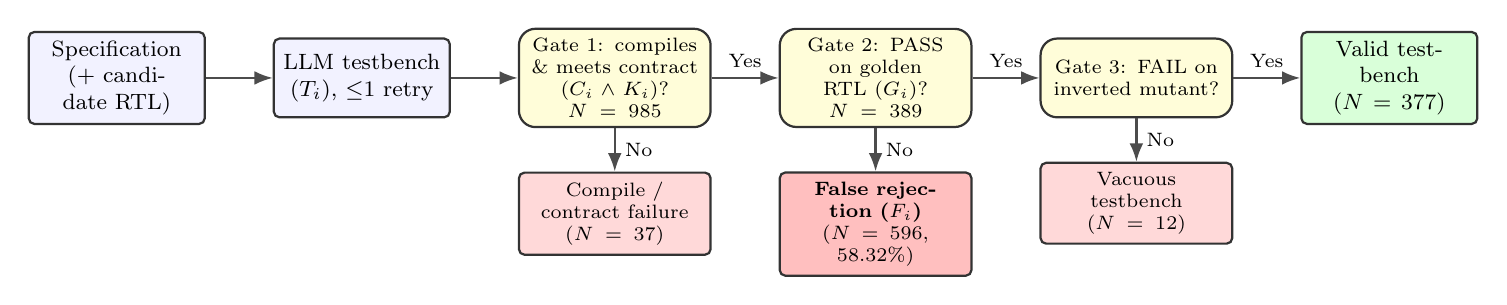
\begin{tikzpicture}[
    node distance=0.55cm and 0.85cm,
    box/.style={rectangle, draw=black!80, fill=blue!5, thick, rounded corners=2pt, text width=2.0cm, minimum height=1.0cm, align=center, font=\footnotesize},
    gate/.style={rectangle, draw=black!80, fill=yellow!15, thick, rounded corners=6pt, text width=2.2cm, minimum height=1.0cm, align=center, font=\scriptsize},
    term/.style={rectangle, draw=black!80, fill=red!15, thick, rounded corners=2pt, text width=2.2cm, minimum height=0.9cm, align=center, font=\scriptsize},
    pass/.style={rectangle, draw=black!80, fill=green!15, thick, rounded corners=2pt, text width=2.0cm, minimum height=1.0cm, align=center, font=\footnotesize},
    arrow/.style={-Latex, thick, draw=black!70}
]

\node[box]  (spec) {Specification (+ candidate RTL)};
\node[box, right=of spec] (gen) {LLM testbench ($T_i$), $\le$1 retry};
\node[gate, right=of gen] (g1) {Gate 1: compiles \& meets contract ($C_i \land K_i$)? \\ $N=985$};
\node[gate, right=of g1]  (g2) {Gate 2: PASS on golden RTL ($G_i$)? \\ $N=389$};
\node[gate, right=of g2]  (g3) {Gate 3: FAIL on inverted mutant?};
\node[pass, right=of g3]  (valid) {Valid testbench\\($N=377$)};

\node[term, below=of g1] (fail_g1) {Compile / contract failure\\($N=37$)};
\node[term, below=of g2, fill=red!25] (fr) {\textbf{False rejection ($F_i$)}\\($N=596$, 58.32\%)};
\node[term, below=of g3] (vac) {Vacuous testbench\\($N=12$)};

\draw[arrow] (spec) -- (gen);
\draw[arrow] (gen) -- (g1);
\draw[arrow] (g1) -- node[above, font=\scriptsize] {Yes} (g2);
\draw[arrow] (g1) -- node[right, font=\scriptsize] {No} (fail_g1);
\draw[arrow] (g2) -- node[above, font=\scriptsize] {Yes} (g3);
\draw[arrow] (g2) -- node[right, font=\scriptsize] {No} (fr);
\draw[arrow] (g3) -- node[above, font=\scriptsize] {Yes} (valid);
\draw[arrow] (g3) -- node[right, font=\scriptsize] {No} (vac);

\end{tikzpicture}%
}
\caption{Three-gate validation pipeline and outcome counts for the 1,022 free-form trials. A testbench is a false rejection ($F_i$) if it passes Gate~1 but reports FAIL on the golden reference RTL at Gate~2. $37 + 596 + 12 + 377 = 1{,}022$.}
\label{fig:pipeline}
\end{figure*}

\subsection{Benchmark Problems}
We screened the first 122 of the 156 VerilogEval-v2 spec-to-RTL problems~\cite{pinckney2024revisiting} and retained those whose golden RTL yields at least eight compilable, non-equivalent mutants (equivalence judged by a 2,000-vector differential simulation); 35 problems qualified and the first 30 in benchmark order were used. This filter removes trivial single-gate problems but also biases the suite toward sequential logic: by the presence of clock edges in the reference RTL, 8 problems are combinational (vector/mux/arithmetic logic and three FSM next-state-logic problems) and 22 are sequential (counters, LFSRs, shift registers, and FSMs). Each problem provides a natural-language specification, a golden reference RTL, and the official VerilogEval testbench. We confirmed that every golden RTL passes its official testbench with zero mismatches under Icarus Verilog~12.0.

\subsection{Execution Environment}
All archived simulations used Icarus Verilog~12.0 (\texttt{iverilog -g2012}, \texttt{vvp}) with a 30-second compile and simulation timeout. For the audit we re-simulated every free-form testbench with Icarus Verilog~12.0 on Linux and, as an independent second engine, with Verilator~5.020 in \texttt{--binary --timing} mode, which supports delay and event controls in testbench processes~\cite{verilator}.

\subsection{Generation Protocol}
Testbenches were requested under a fixed contract: module \texttt{tb}, DUT instance \texttt{TopModule dut}, outputs compared with \texttt{!==}, a standardized \texttt{MISMATCH} line per failed check, and exactly one \texttt{*** TEST RESULT: PASS ***} or \texttt{FAIL} line before \texttt{\$finish}. If the first attempt failed to compile or violated the contract on the golden RTL, the model received the error and one retry (used in 75 of 1,022 trials). Candidate RTL was generated once per (problem, generator, sample) with one compile-error retry and reused across conditions. All models used temperature 0.2 and a 2,048-token output limit. Each configuration was sampled three times; the sample labels (42, 43, 44) enter the response-cache key but are not passed to the OpenAI or Gemini APIs, so the three samples are independent draws rather than seeded replays.

\subsection{Archived Arms}
The archive contains 1,112 trials in two arms. In a \textit{template pilot} ($N=90$) the harness supplied the module shell, clock, reset, and DUT instance, and the model wrote only stimulus statements; 75 testbenches failed to compile and the remaining 15 passed the golden RTL but were vacuous, so the arm produced no valid testbench and no false rejection and is excluded from analysis. The \textit{free-form arm} ($N=1{,}022$), in which the model writes the complete testbench, is the evaluation corpus.

\subsection{Conditions}
Let $G$ be the model that generated the candidate RTL and $T$ the other cloud model. The six conditions are:
\begin{itemize}
    \item \textbf{A (Self-test):} $G$ writes the testbench from the specification and candidate RTL using a neutral ``verification engineer'' prompt.
    \item \textbf{B (Same-model adversary):} $G$ itself, prompted as an adversarial red-team engineer, sees specification and candidate RTL. (The configuration file names this ``same-family'', but for both cloud pairings $G'$ is the same model checkpoint as $G$; B therefore differs from A only in the prompt.)
    \item \textbf{B$'$ (Same-model adversary, spec only):} as B, with the candidate RTL withheld.
    \item \textbf{C (Cross-model adversary):} $T$ with the adversarial prompt, specification, and candidate RTL.
    \item \textbf{C$'$ (Cross-model adversary, spec only):} as C, with the candidate RTL withheld.
    \item \textbf{D (Self-test resample):} identical to A with an independent sample. The pipeline was designed to make D compute-matched to C, but as implemented it issues a single request with the same prompt and retry budget as A (mean tester tokens 1,811 vs.\ 1,812). We therefore treat D as a test--retest replicate of A, which directly measures sampling noise.
\end{itemize}
These conditions span three prompt types (neutral self, adversarial with RTL, adversarial spec-only) crossed with whether the testbench author is the RTL generator. Because each cloud model generates RTL for its own problems and tests the other model's RTL in C and C$'$, both models act as testbench authors in every condition.

\subsection{Models and Trial Allocation}
\begin{itemize}
    \item \textbf{GPT-4o-mini} (\texttt{gpt-4o-mini-2024-07-18}): generator in 540 trials (all 30 problems) and testbench author in 514.
    \item \textbf{Gemini Flash-Lite} (requested as \texttt{gemini-3.5-flash-lite}): generator in 462 trials (26 problems; not Prob110, Prob111, Prob114, Prob115) and testbench author in 488 (all 30 problems). The client's fallback model \texttt{gemini-3.8-flash} served 6 generation and 5 testbench calls, and 60 trials from an early pilot have no recorded model version.
    \item \textbf{Local pilot:} \texttt{qwen2.5-coder:1.5b} generated RTL and \texttt{llama3.1:8b} wrote all testbenches for 20 trials on Prob006 (18) and Prob021 (2). Because the tester is \texttt{llama3.1:8b} in every condition, including the nominal self-test conditions A and D, the condition labels do not apply to these trials. They are included in prevalence estimates (RQ1, RQ3) and excluded from condition and model analyses, which use the 1,002 cloud trials.
\end{itemize}

\subsection{Statistical Methods}
Trials are clustered within 30 problems. The ANOVA estimator gives an intraclass correlation of $\rho = 0.2665$ for the false-rejection indicator; with mean cluster size $\bar{m} = 34.07$ the design effect is $D_{\text{eff}} = 1 + (\bar{m}-1)\rho = 9.81$, an effective sample size of about 104 trials. We therefore report Wilson score intervals~\cite{wilson1927probable} only as descriptive trial-level intervals and base inference on (i) a problem-level cluster bootstrap~\cite{cameron2015practitioner, efron1994introduction} (10,000 resamples of whole problems, seed 42), (ii) problem-level paired comparisons with bootstrap CIs and sign-flip permutation tests (10,000 draws), and (iii) a logistic generalized estimating equation (GEE)~\cite{liang1986longitudinal} with problem clusters and an exchangeable working correlation. The omnibus Pearson $\chi^2$ test~\cite{pearson1900criterion} across conditions ignores clustering and is reported for completeness; because it is anti-conservative, a non-significant result is all the more informative. All numbers in this paper are produced by \texttt{paper/audit/analysis.py}.

\section{Results}

\begin{table*}[t]
\centering
\caption{False-rejection rates across problem subsets (all 1,022 free-form trials). ``Gate~1'' rows condition on testbenches that compile and meet the contract ($C_i \land K_i$, including the 12 vacuous testbenches, which pass the golden RTL). Cluster bootstrap: 10,000 problem-level resamples, seed 42.}
\label{tab:headline_rates}
\footnotesize
\setlength{\tabcolsep}{4pt}
\begin{tabular}{lcccccc}
\toprule
\textbf{Subset} & \textbf{Problems} & \textbf{Trials ($N$)} & \textbf{$F_i$} & \textbf{Rate (\%)} & \textbf{Wilson 95\% CI} & \textbf{Cluster Bootstrap 95\% CI} \\
\midrule
All trials & 30 & 1,022 & 596 & \textbf{58.32} & [55.27, 61.30] & [48.69, 67.72] \\
Gate~1 passed & 30 & 985 & 596 & \textbf{60.51} & [57.42, 63.51] & [51.50, 69.11] \\
\midrule
Excl.\ 2 port-inconsistent problems & 28 & 950 & 539 & \textbf{56.74} & [53.57, 59.85] & [46.49, 66.45] \\
\quad Gate~1 passed & 28 & 914 & 539 & \textbf{58.97} & [55.75, 62.12] & [49.38, 67.81] \\
Excl.\ all 3 flagged problems & 27 & 914 & 505 & \textbf{55.25} & [52.01, 58.45] & [44.91, 64.97] \\
\midrule
Combinational & 8 & 290 & 98 & \textbf{33.79} & [28.59, 39.42] & [18.39, 50.00] \\
\quad Gate~1 passed & 8 & 254 & 98 & \textbf{38.58} & [32.81, 44.70] & [22.34, 54.08] \\
Sequential & 22 & 732 & 498 & \textbf{68.03} & [64.57, 71.31] & [59.19, 76.09] \\
\quad Gate~1 passed & 22 & 731 & 498 & \textbf{68.13} & [64.66, 71.40] & [59.26, 76.26] \\
\midrule
6 clean combinational (post hoc) & 6 & 218 & 54 & \textbf{24.77} & [19.51, 30.90] & [9.89, 40.74] \\
\quad Gate~1 passed & 6 & 187 & 54 & \textbf{28.88} & [22.86, 35.75] & [12.35, 45.26] \\
4 simple combinational (post hoc) & 4 & 146 & 18 & \textbf{12.33} & [7.94, 18.65] & [1.79, 18.89] \\
\quad Gate~1 passed & 4 & 118 & 18 & \textbf{15.25} & [9.87, 22.83] & [2.50, 21.79] \\
\bottomrule
\end{tabular}
\end{table*}

\subsection{RQ1: Prevalence and Simulator Robustness}
Of 1,022 free-form testbenches, 7 failed to compile and 30 violated the output contract on the golden RTL, leaving 985 (96.38\%) that passed Gate~1 (Fig.~\ref{fig:pipeline}). Only 389 of these reported PASS on the golden RTL, and 12 of those also passed the inverted-output mutant and were rejected as vacuous, leaving 377 valid testbenches (36.89\%). The remaining 596 trials are false rejections:
\begin{equation}
\text{FRR}_{\text{all}} = \frac{596}{1{,}022} = 58.32\%, \qquad \text{FRR}_{\text{G1}} = \frac{596}{985} = 60.51\%,
\end{equation}
with problem-level cluster bootstrap CIs of [48.69\%, 67.72\%] and [51.50\%, 69.11\%]. Restricting to the 1,002 cloud trials gives 58.88\% (590/1,002).

\textit{Reproduction.} We re-ran every free-form testbench against the golden RTL and the inverted-output mutant under Icarus Verilog~12.0 on a different host and operating system. All 1,022 archived verdicts (compile failure, contract violation, FAIL, PASS, vacuous) were reproduced exactly.

\textit{Second simulator.} \VERILATORRESULTS

\subsection{RQ2: Prompting Role Does Not Move the Rate}
Table~\ref{tab:conditions} gives outcomes for the 1,002 cloud trials. Rates lie between 55.69\% and 62.87\%, and the omnibus test is far from significance ($\chi^2 = 3.15$, $df = 5$, $p = 0.68$). Problem-level paired comparisons (30 problems) isolate individual factors:
\begin{itemize}
    \item \textit{Sampling noise} (D$-$A, identical configuration): $-1.44$ pp, 95\% CI [$-11.67$, $7.78$].
    \item \textit{Adversarial prompt} (B$-$A, same model and inputs): $+7.22$ pp, [$-1.11$, $16.67$], $p = 0.18$.
    \item \textit{Hiding the candidate RTL} (B$'-$B): $-3.78$ pp, [$-14.11$, $6.33$], $p = 0.54$; (C$'-$C): $+2.44$ pp, [$-5.11$, $10.00$], $p = 0.59$.
    \item \textit{Cross-model checker} (C$-$B, same prompt): $-6.78$ pp, [$-15.78$, $2.56$], $p = 0.17$.
\end{itemize}
The A--D replicate shows that, with three samples per problem, condition-level differences of up to about $\pm 10$ pp are within sampling noise; none of the designed contrasts exceeds that band.

\begin{table}[t]
\centering
\caption{Outcomes by condition (1,002 cloud trials). Each condition has 90 GPT-4o-mini and 77 Gemini Flash-Lite testbench authors; Gate-1 counts include vacuous testbenches.}
\label{tab:conditions}
\footnotesize
\setlength{\tabcolsep}{3pt}
\begin{tabular}{lcccrc}
\toprule
\textbf{Cond.} & \textbf{$N$} & \textbf{Pass G1} & \textbf{$F_i$} & \textbf{Rate (\%)} & \textbf{Wilson 95\% CI} \\
\midrule
A (Self)          & 167 & 159 & 93  & 55.69 & [48.11, 63.01] \\
B (Same+RTL)      & 167 & 161 & 105 & 62.87 & [55.33, 69.84] \\
B$'$ (Same-Spec)  & 167 & 164 & 102 & 61.08 & [53.51, 68.14] \\
C (Cross+RTL)     & 167 & 159 & 96  & 57.49 & [49.90, 64.73] \\
C$'$ (Cross-Spec) & 167 & 164 & 101 & 60.48 & [52.91, 67.58] \\
D (Resample of A) & 167 & 161 & 93  & 55.69 & [48.11, 63.01] \\
\bottomrule
\end{tabular}

\vspace{3pt}
\begin{minipage}{0.96\columnwidth}
\scriptsize
Pearson $\chi^2 = 3.15$, $df = 5$, $p = 0.68$. Problem-level paired permutation: B$-$A $+7.22$ pp ($p = 0.18$); C$-$B $-6.78$ pp ($p = 0.17$); D$-$A $-1.44$ pp ($p = 0.84$).
\end{minipage}
\end{table}

\subsection{RQ3: Circuit Type and Specification Defects}
\subsubsection{Combinational vs.\ sequential}
False rejections are concentrated in sequential problems (68.03\%, cluster CI [59.19\%, 76.09\%]) relative to combinational ones (33.79\%, [18.39\%, 50.00\%]) (Table~\ref{tab:headline_rates}). Per-problem rates range from 0\% (\texttt{Prob114\_bugs\_case}) to 94.4\% (\texttt{Prob040\_count10}, \texttt{Prob068\_countbcd}, \texttt{Prob088\_ece241\_2014\_q5b}). With only eight combinational problems, this contrast is between small groups of problems and should not be read as a per-circuit causal effect.

\subsubsection{Specification defects}\label{sec:specdefects}
Comparing each specification with its reference RTL, we flagged three problems:
\begin{enumerate}
    \item \texttt{Prob068\_countbcd}: the specification declares \texttt{ena} as 4 bits, while the reference declares \texttt{ena[3:1]} (3 bits); the prose (``for digits [3:1]'') matches the reference.
    \item \texttt{Prob099\_m2014\_q6c}: the specification declares a 7-bit \texttt{y} and asks for next-state signals \texttt{Y2} and \texttt{Y4}, while the reference has a 6-bit \texttt{y} and ports \texttt{Y1}, \texttt{Y3}.
    \item \texttt{Prob088\_ece241\_2014\_q5b}: the specification asks for a one-hot encoding while the reference uses a binary state register. Because state encoding is not observable at the ports, this mismatch cannot by itself cause a false rejection; we report it separately.
\end{enumerate}
The two problems with port-level contradictions account for 57 of their 72 trials (79.17\%). Excluding them lowers the overall rate by only 1.58 pp, to 56.74\% (cluster CI [46.49\%, 66.45\%]); excluding all three gives 55.25\%. Specification defects inflate false rejections on the affected problems, but they do not explain the overall rate.

\subsubsection{Post hoc combinational subsets}
Removing \texttt{Prob099} (port-inconsistent) and \texttt{Prob043\_vector5} leaves six combinational problems with a 24.77\% rate (54/218). \texttt{Prob043}'s specification is consistent with its reference (the bit ordering is fixed by an example), so its exclusion is a post hoc choice rather than a specification defect; including it raises the rate to 33.79\% (all eight combinational problems). Two of these (\texttt{Prob091}, \texttt{Prob100}) describe FSM next-state logic; the remaining four purely datapath problems (\texttt{Prob006}, \texttt{Prob021}, \texttt{Prob033}, \texttt{Prob114}) still have a 12.33\% rate (18/146, cluster CI [1.79\%, 18.89\%]). These subsets were defined after seeing the data and are exploratory.

\begin{figure}[t]
\centering
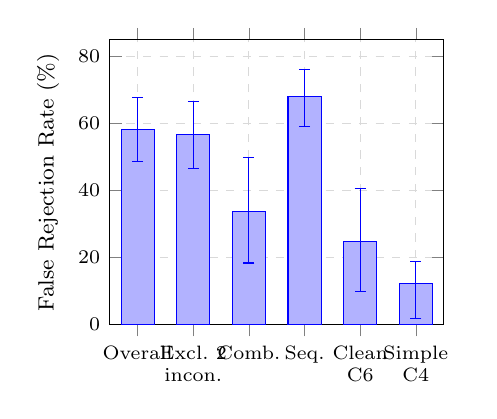
\begin{tikzpicture}
\begin{axis}[
    ybar,
    bar width=12pt,
    width=0.48\textwidth,
    height=5.2cm,
    ymin=0,
    ymax=85,
    ylabel={False Rejection Rate (\%)},
    symbolic x coords={All, Excl-Incon, Comb, Seq, Clean-Comb, Simple-4},
    xtick=data,
    xticklabels={Overall, Excl.\ 2 incon., Comb., Seq., Clean C6, Simple C4},
    x tick label style={font=\scriptsize, align=center, text width=1.1cm},
    y tick label style={font=\scriptsize},
    ylabel style={font=\footnotesize},
    grid=major,
    grid style={dashed, gray!30},
]

\addplot+[error bars/.cd, y dir=both, y explicit]
coordinates {
    (All, 58.32)        += (0, 9.40)  -= (0, 9.63)
    (Excl-Incon, 56.74) += (0, 9.71)  -= (0, 10.25)
    (Comb, 33.79)       += (0, 16.21) -= (0, 15.40)
    (Seq, 68.03)        += (0, 8.06)  -= (0, 8.84)
    (Clean-Comb, 24.77) += (0, 15.97) -= (0, 14.88)
    (Simple-4, 12.33)   += (0, 6.56)  -= (0, 10.54)
};

\end{axis}
\end{tikzpicture}
\caption{False-rejection rates across problem groupings with 95\% problem-level cluster bootstrap confidence intervals (all 1,022 free-form trials).}
\label{fig:rates_chart}
\end{figure}

\subsection{RQ4: Tester Identity Dominates}
\subsubsection{Testbench author}
Pooling over conditions, GPT-4o-mini testbenches falsely reject the golden design in 382 of 514 trials (74.32\%, Wilson [70.37\%, 77.91\%]) and Gemini Flash-Lite testbenches in 208 of 488 (42.62\%, [38.31\%, 47.05\%]). The gap holds within each prompt type (Table~\ref{tab:tester}, Fig.~\ref{fig:tester}) and at the problem level: across the 30 problems the mean per-problem rate is 72.87\% vs.\ 41.64\%, a paired difference of $-31.23$ pp (95\% bootstrap CI [$-42.59$, $-20.21$], permutation $p < 10^{-4}$); excluding the two port-inconsistent problems gives $-31.28$ pp ([$-42.89$, $-20.17$]).

A problem-clustered logistic GEE with tester identity, prompt type, and a same-model indicator (tester is also the RTL generator) gives:
\begin{itemize}
    \item GPT-4o-mini vs.\ Gemini Flash-Lite tester: OR $= 4.13$ [2.50, 6.81], $p < 0.001$;
    \item adversarial prompt with RTL vs.\ neutral self prompt: OR $= 1.32$ [0.99, 1.75], $p = 0.058$;
    \item adversarial spec-only prompt vs.\ neutral self prompt: OR $= 1.35$ [1.02, 1.79], $p = 0.035$;
    \item tester is the RTL generator (self vs.\ cross-model): OR $= 1.01$ [0.78, 1.32], $p = 0.94$.
\end{itemize}
Testing one's own design rather than the other model's design therefore makes no difference once the tester's identity is accounted for, and the adversarial ``red-team'' framing, if anything, slightly increases false rejections.

\subsubsection{RTL generator}
Grouping trials by the model that generated the candidate RTL gives a smaller difference (26 shared problems: 65.81\% for GPT-4o-mini vs.\ 55.34\% for Gemini Flash-Lite, $-10.47$ pp, CI [$-16.67$, $-4.27$]). This apparent generator effect is entirely a tester effect: four of six conditions use the generator as tester. Holding the tester fixed and restricting to prompts that show the RTL, the generator of the shown RTL changes the rate by $-0.64$ pp for GPT-4o-mini testers (CI [$-9.62$, $8.33$]) and $-1.50$ pp for Gemini Flash-Lite testers ([$-13.25$, $9.19$]).

\begin{table}[t]
\centering
\caption{False rejections by testbench author and prompt type (1,002 cloud trials), $k/n$ (\%). ``Self'' pools A and D; Gemini F-L = Gemini Flash-Lite.}
\label{tab:tester}
\footnotesize
\setlength{\tabcolsep}{4pt}
\begin{tabular}{lccc}
\toprule
\textbf{Prompt} & \textbf{GPT-4o-mini} & \textbf{Gemini F-L} & \textbf{Diff.\ (pp)} \\
\midrule
Self (A, D)            & 125/180 (69.4) & 61/154 (39.6) & $-29.8$ \\
Adv.\ + RTL (B, C)     & 123/167 (73.7) & 78/167 (46.7) & $-26.9$ \\
Adv.\ spec (B$'$, C$'$) & 134/167 (80.2) & 69/167 (41.3) & $-38.9$ \\
\midrule
All                    & 382/514 (74.3) & 208/488 (42.6) & $-31.7$ \\
\bottomrule
\end{tabular}
\end{table}

\begin{figure}[t]
\centering
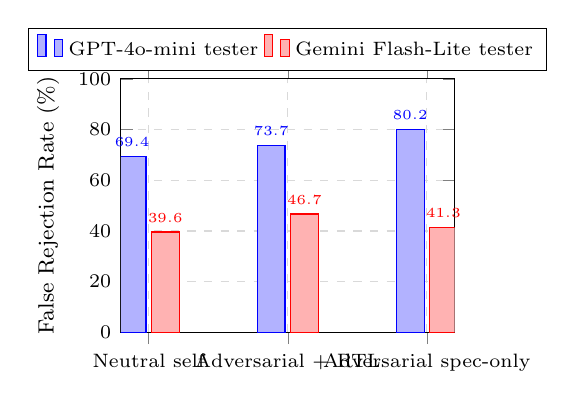
\begin{tikzpicture}
\begin{axis}[
    ybar,
    bar width=10pt,
    width=0.48\textwidth,
    height=4.8cm,
    ymin=0, ymax=100,
    ylabel={False Rejection Rate (\%)},
    symbolic x coords={Self, AdvRTL, AdvSpec},
    xtick=data,
    xticklabels={Neutral self, Adversarial + RTL, Adversarial spec-only},
    x tick label style={font=\scriptsize},
    y tick label style={font=\scriptsize},
    ylabel style={font=\footnotesize},
    legend style={at={(0.5,1.03)}, anchor=south, legend columns=2, font=\scriptsize},
    nodes near coords, nodes near coords style={font=\tiny},
    grid=major, grid style={dashed, gray!30},
]
\addplot coordinates {(Self, 69.4) (AdvRTL, 73.7) (AdvSpec, 80.2)};
\addplot coordinates {(Self, 39.6) (AdvRTL, 46.7) (AdvSpec, 41.3)};
\legend{GPT-4o-mini tester, Gemini Flash-Lite tester}
\end{axis}
\end{tikzpicture}
\caption{False-rejection rate by testbench author and prompt type. The tester gap (about 30 pp) is several times larger than any prompt effect.}
\label{fig:tester}
\end{figure}

\subsubsection{Anchoring on buggy candidates}
For each testbench we also simulated the candidate RTL it was written for. Among Gate-1 testbenches written for a candidate that fails the official VerilogEval testbench, 31 of 194 written with the candidate RTL visible (16.0\%) rejected the golden design \textit{and} passed the buggy candidate, compared with 8 of 98 (8.2\%) written from the specification alone. Such a testbench would lead a repair loop to accept the bug and reject the fix. A GEE with an interaction between candidate correctness and RTL visibility points in the same direction but is not significant (interaction OR $= 1.54$ [0.89, 2.68], $p = 0.12$), so we treat anchoring as a plausible but unconfirmed mechanism.

\section{Qualitative Failure Analysis}
Only 6 of the 596 false-rejecting testbenches emitted the requested standardized \texttt{MISMATCH} line; the rest used free-form error messages. Automated classification of the first mismatch is therefore unreliable: on a manually labeled sample of 25 false rejections, the pipeline's rule-based categories agreed with manual labels in 16 cases (64\%). We therefore report only mechanisms visible directly in simulator output.

\subsection{Cycle Alignment of Sequential Expectations}
In counters and shift registers, many testbenches expect a register value one cycle early or late. For example, in \texttt{Prob040\_count10} (94.4\% false rejection) typical logs show the testbench's expected count sequence shifted by one or two counts relative to the golden output at every subsequent check (e.g., ``Expected q = 2, got q = 1'', ``q = 0010, expected = 0000''), consistent with sampling outputs at the active clock edge, before the non-blocking update, or miscounting the reset cycle.

\subsection{Checking Before Reset Takes Effect}
In 52 of the 596 false rejections (8.7\%), the golden design's output was still \texttt{X} at the failing check (e.g., ``Expected q = 1, got q = xxxx'' in \texttt{Prob035\_count1to10}), meaning the testbench checked an output before applying or completing the synchronous reset. All 596 testbenches used the case-inequality operator \texttt{!==}, so these failures are sequencing errors in the stimulus, not artifacts of 2-state comparisons.

\subsection{Under-Specified Conventions}
Some specifications leave conventions implicit. \texttt{Prob060\_m2014\_q4k} (``a shift register with four D flops'') does not state the shift direction or which flop drives \texttt{out}, and has a 61.1\% false-rejection rate. In contrast, \texttt{Prob085\_shift4} states the direction explicitly (``shift right (q[3] becomes zero, q[0] is shifted out)'') and has one of the lowest sequential rates (19.4\%), which suggests that explicit specification of conventions helps.

\section{Threats to Validity}
\begin{enumerate}
    \item \textit{Oracle validity.} Golden RTL designs are from VerilogEval-v2 and pass their official testbenches, but they are not formally proven equivalent to the prose specifications; two problems contain port-level contradictions (Section~\ref{sec:specdefects}). In 14 false rejections the testbench also passed a candidate that passes the official testbench, which indicates either uncovered differences between candidate and golden behavior or limited coverage of the official testbench.
    \item \textit{Simulator dependence.} \VERILATORTHREAT
    \item \textit{Model coverage and versions.} Only two cloud models were evaluated as testbench authors, so ``tester identity'' is a comparison of two models, not of model families. Model versions were not recorded for 60 pilot trials, and 11 calls were served by a fallback Gemini model. The 20 local-model trials are too few to support model-level conclusions.
    \item \textit{Design of conditions.} The planned compute-matched control (D) was implemented as a resample of A, so this study does not test whether a larger self-testing budget closes any gap. Condition B uses the same checkpoint as A, not a distinct same-family model.
    \item \textit{Sampling.} Three samples per configuration at temperature 0.2 provide limited within-configuration replication; the A--D replicate bounds the resulting noise at roughly $\pm 10$ pp per condition.
    \item \textit{Problem selection.} The $\ge 8$-mutant filter favors sequential problems and excludes the simplest benchmarks; prevalence estimates apply to this filtered subset.
\end{enumerate}

\section{Conclusion}
Across 1,022 LLM-written Verilog testbenches, 58\% reject a correct reference design despite compiling and following the output contract, and this measurement is reproducible across simulators. Prompting strategies that are often proposed as remedies---adversarial red-team framing, hiding the implementation, or checking with a different model under the same prompt---do not reduce the rate beyond sampling noise. The single largest factor is which model writes the testbench: one of the two evaluated models produced false rejections at roughly 1.7 times the rate of the other. For closed-loop RTL generation, this suggests that (i) LLM-generated testbenches must themselves be validated, for example against a trusted reference model or by cross-checking several testbenches, before their verdicts are allowed to drive repairs; (ii) testbench-writing models should be benchmarked on false rejection directly, since role prompting does not substitute for a better tester; and (iii) sequential timing and reset conventions should be stated explicitly in specifications given to LLM testbench writers.

\bibliographystyle{IEEEtran}
\bibliography{references}

\end{document}
